% This is LLNCS.DEM the demonstration file of
% the LaTeX macro package from Springer-Verlag
% for Lecture Notes in Computer Science,
% version 2.4 for LaTeX2e as of 16. April 2010
%
\documentclass{llncs}
%
\usepackage{amsmath}
\usepackage{amssymb}
\usepackage{tikz}

\newcounter{instr}
\newcommand{\ninstr}{\refstepcounter{instr}\theinstr.}

\begin{document}

\title{Species delimitation}

\titlerunning{Species delimitation}

\author{Tom\'{a}\v{s} Flouri1\inst{1} \and Paschalia Kapli\inst{1} \and Sarah Lutteropp\inst{1}}
\authorrunning{Tom\'{a}\v{s} Flouri et al.} % abbreviated author list
\institute{Heidelberg Institute of Theoretical Studies}

\maketitle

\begin{abstract}
An explanation of the single-lambda and multiple-lambda heuristic for PTP.
\end{abstract}

\section{Related Work}

The heuristic is based on a similar idea as the algorithm from Gulek et al.\cite{Gulek:2010:DPA:1838770.1839019} for the tree-like weighted set packing problem.

\ldots

\section{Task Description}

Given a rooted fully binary tree with non-negative edge weight function $w$, we want to partition its leaves into disjoint sets (called species). The \emph{most recent common ancestors} (MRCA) of those species induce subtrees with edge sets $E_1, \ldots, E_{k}$. Every edge that is not assigned to one of those subtrees is then put into the set of speciation edges, $E_{k+1}$.

Given a set of edges $E$, we define its log-likelihood $logl(E)$ as
$$logl(E) := |E| * (\log{|E|} - 1 - \log{\sum_{e \in E} w(e)})$$

\paragraph{Multiple Lambda Score}

We want to find a delimitation such that the following sum of loglikelihoods (in the following referred to as \emph{score}) is maximized:

$$\sum_{i=1}^{k+1}{logl(E_i)}$$

\paragraph{Single Lambda Score}

We want to find a delimitation such that the following sum of loglikelihoods (in the following referred to as \emph{score}, too) is maximized:

$$logl(\cup_{i=1}^k{E_i}) + logl(E_{k+1})$$

\section{General Idea}

We follow a bottom-up dynamic programming approach, always trying to extend a good solution for the children subtrees in order to obtain a good solution for the currently observed tree.

\subsection{Currently observed tree}

For each node $v$, the \emph{currently observed tree} (COT) consists of the subtree rooted at $v$, $S(v)$, and the set of edges where we already know that they have to be speciation edges in the case that a node in $S(v)$ is a speciation event (see Fig.~\ref{fig:currently_observed_tree}). Our aim is to find a delimitation that yields to a high score for the COT. This means that every edge that is not contained in the COT will be ignored by the score computation since we do not know its assignment.

\begin{figure}[h!]
	\centering
	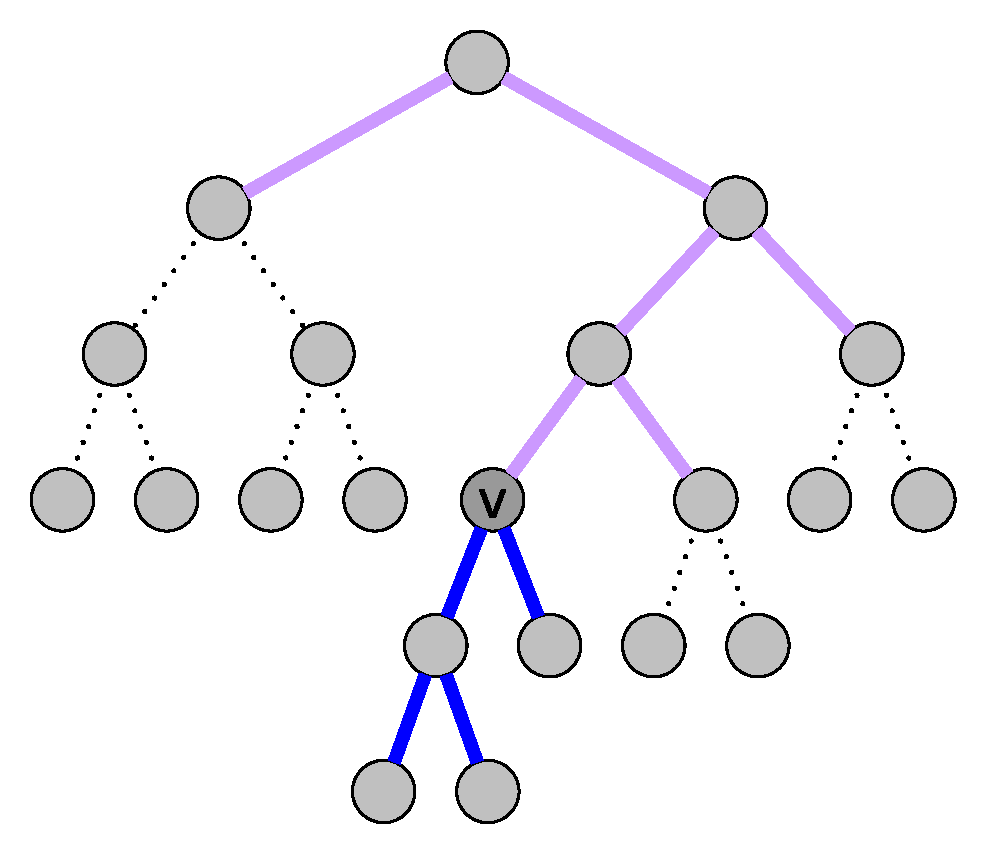
\includegraphics[scale=0.4]{images/currently_observed_tree.pdf}
	\caption{The currently observed tree of $v$, marked with thick blue edges}
	\label{fig:currently_observed_tree}
\end{figure}

\subsection{Combination of solutions}

For every node, we store an array that contains the best found score for $0, 2, 4, \ldots$ speciation edges and the delimitation that led to it.

\paragraph{Zero speciation edges}
If we have $0$ speciation edges in $S(v)$, it simply means that $v$ is handled as the root of a coalescent group (species). Thus we can directly use the score function to obtain this score and do not need to look at the children's scores.

\paragraph{More than zero speciation edges}
In order to find a solution for a subtree $S(v)$ and $k>0$ speciation edges, we combine the best found solution for $i$ speciation edges from the left child of $v$ with the best found solution for $j$ speciation edges for the right child of $v$ for all choices of $i$ and $j$ where $i+j+2$ sums up to $k$ (see Fig.~\ref{fig:combining}). We compute the score of the combined delimitation using either the single-lambda or multiple-lambda approach. Then we store the delimitation that yields to the highest score for $k$ speciation edges inside $v$.

\begin{figure}[h!]
\centering
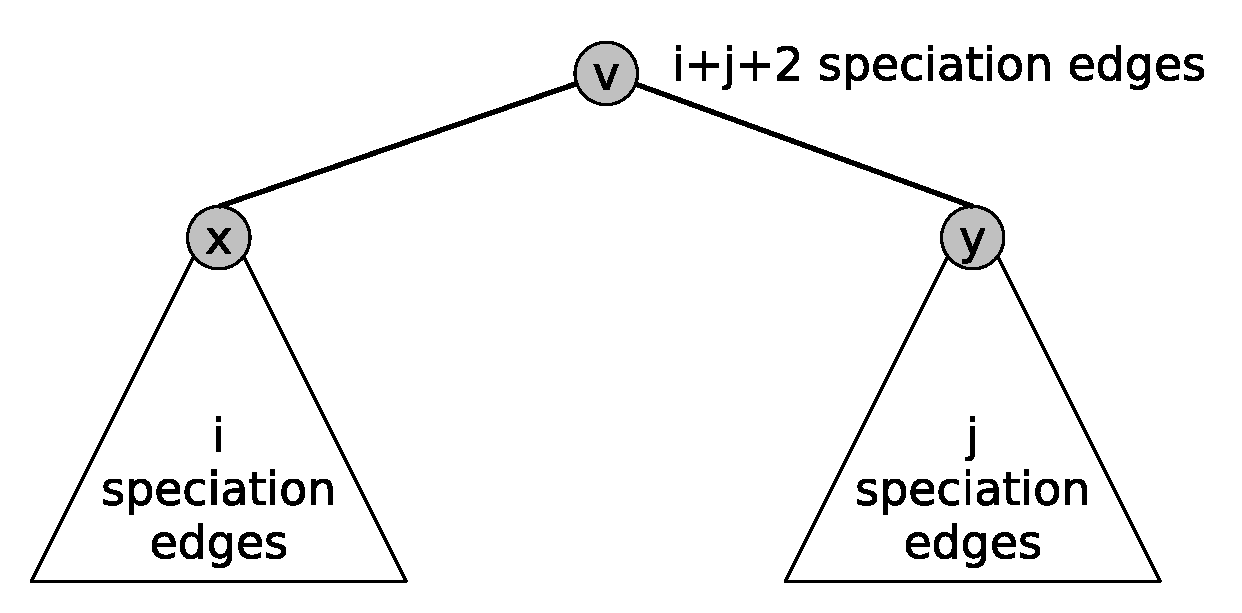
\includegraphics[scale=0.3]{images/speciation_events.pdf}
\caption{Combining the best found solutions for the subtrees}
\label{fig:combining}
\end{figure}

\section{Handling of zero-length Edges}

If the sum of edge-weights in a subtree is zero, its corresponding log-likelihood value would be infinity. Because this worsens the delimitation results a lot, we decide to treat this case differently.

Since a subtree with edge sum zero originates from identical sampled sequences, we shrink the whole subtree to a single node, thus reducing the total number of edges in the tree.

Other zero-length edges that may appear in the tree (e.g., for representing multifurcations) are not treated differently as they do not cause any problems.

(TODO: image with zero length edges)

\bibliographystyle{splncs03}
\bibliography{delimit}
\end{document}
